\documentclass[letterpaper,12pt,oneside]{article}

\usepackage[utf8]{inputenc}
\usepackage[spanish,es-nodecimaldot,es-tabla]{babel}
\usepackage{graphicx}
\usepackage{array}
\usepackage{natbib}
\bibliographystyle{plain}

\title{Detección temprana de somnolencia en conductores automovilistas mediante el seguimiento ocular: análisis específico del parpadeo lento}
\author{Brandon Garay Jacome}
\date{Marzo 2025}

\begin{document}

\maketitle

\section*{Resumen}
En el mundo tan agitado en el que vivimos muchas personas tienden a demeritar la importancia del sueño trayendo consigo graves consecuencias , una de ellas el ocasionar accidentes automovilísticos. \cite{torre}. Actualmente, existen soluciones tecnológicas para la detección de somnolencia, basadas en análisis de patrones de conduccion, sensores fisiológicos y seguimiento ocular.\cite{EspinolaGonzales2011,MendietaZrate2018} Sin embargo, las soluciones basadas en el seguimiento ocular suelen enfocarse en metricas generales, como la frecuencia de parpadeo o el cierre prolongado de los ojos, sin un analisis profundo del parpadeo lento, un indicador mas sutil y temprano de la fatiga.

Esta investigacion propone un sistema de detección temprana de somnolencia en conductores mediante el analisis especifico del parpadeo lento utilizando técnicas de visión artificial con MediaPipe y métricas personalizadas de seguimiento ocular. Se espera que esta propuesta contribuya a una mayor precisión en la detección temprana de la fatiga al volante, ayudando a reducir accidentes de trafico relacionados con la somnolencia. Además, se plantea una comparación con las soluciones existentes, evaluando la efectividad y las limitaciones existentes.




\section{Objetivos}

\subsection{Objetivo general}
Desarrollar un prototipo de deteccion temparana de somnolencia en conductores mediante el analisis especifico del parpadeo lento utilizando tecnicas de vision artificial con MediaPipe.




\subsection{Objetivos particulares}
Se busca investigar y plantear una metodología de detección temprana de somnolencia temprana tomando como principal determinante el parpadeo lento.

Se buscara implementar algoritmos de seguimiento ocular con apoyo de la herramienta de MediaPipe para monitorear el parpadeo del conductor.

Desarrollar un modelo para identificar el parpadeo lento mediante métricas personalizadas del Aspecto de Relación Ocular.

Evaluar la efectividad del prototipo propuesto para la detección de somnolencia temprana.

Validar el sistema en escenarios simulados de conducción para garantizar su fiabilidad.



\section{Definición del Problema}
Según la OMS los transtornos del sueño afectan al 40\%  de la población, en muchos países esto genera la principal causa de muerte por accidentes automovilísticos, De acuerdo a una investigación realizada por la Clínica de Trastornos del Sueño de la UNAM, en nuestro país alrededor del 45\% de la población adulta presenta mala calidad del sueño.\cite{capufe_sleep}.

Para ello se ha tratado de implementar diversas herramientas tecnológicas que ayuda a evitar accidentes causados por somnolencia. Sin embargo, muchas de ellas, especialmente aquellas enfocadas en el reconocimiento de somnolencia en tiempo real, solo detectan signos evidentes, como los cabeceos, los cuales suelen manifestarse en etapas avanzadas del problema. por ello se busca la implementación de una metodología que pueda detectar este problema de manera temprana.
 



\section{Metodología}

Para poder implementar un prototipo capaz de detectar de manera temprana la somnolencia en conductores mediante el análisis del parpadeo lento, se seguirá un enfoque metodológico basado en el reconocimiento de patrones oculares. Para ello, se diseñarán algoritmos y software capaces de estudiar el comportamiento ocular en sus etapas iniciales en tiempo real. Finalmente, el sistema será validado para garantizar su precisión y eficacia.

%\subsection{Proceso Científico-metodológicos }
\begin{enumerate}
    \item \textbf{Revisión de Literatura}
    \begin{itemize}
        \item Analisis de estudios previos centrados en la deteccion de somnolencia.
        \item Tecnicas de reconocimiento ocular.
        \item Algoritmos implementados para la deteccion  de somnolencia
    \end{itemize}
    \item \textbf{Selección de Tecnologia}
    \begin{itemize}
        \item Identificar librerias y herramientas que se implementaran en el software.
        \item Determinar el hardware necesario que se ocupara al igual que sus requerimientos
    \end{itemize}
    \item \textbf{Boceto de Prototipo}
    \begin{itemize}
         \item Identificar parametros a medir.
        \item  Determinar los parametros adecuados para una mejor deteccion de datos (Posición , orientación de la camara)
        
    \end{itemize}
    \item \textbf{Desarrollo e implementación}
    \begin{itemize}
        \item Con la informacion recopilada y los parametros del boceto, desarrollar el prototipo.
        \item Imelementar las herramientas que mejor se adapten a nuestro objetivo.
        
    \end{itemize}
    \item \textbf{Validacion }
    \begin{itemize}
        \item Se haran diversas pruebas para identificar como es el comportamiento del prototipo.
        \item Evaluación de resultados.
    \end{itemize}
    
\end{enumerate}





\section{Inventario de materias/temas de la carrera que se utilizarán para el desarrollo de seminario / tesis}


\begin{itemize}
    \item Fundamentos de programación
    \begin{itemize}
        \item Resolución de problemas 
        \item Fundamentos para la construcción de código a partir del algoritmo
        \item Paradigmas de programación
    \end{itemize}
    \item Reconocimiento  de Patrones
    \begin{itemize}
        \item Segmentacion de patrones faciales especificos 
        \item Implementacion de redes neuronales convolucionales
    \end{itemize}
    \item Ingenieria de Software
    \begin{itemize}
        \item Metodologia de creacion de software 
        \item Buenas practicas en la documentacion de codigo
    \end{itemize}
    
\end{itemize}

\section{Índice desglosado de la tesis}
El índice propuesto de la tesis con secciones y subsecciones.

\begin{enumerate}
    \item Introducción
    \item Marco teórico
    \item Análisis del problema
    \item Diseño de solución
    \item Implementación
    \item Resultados y pruebas
    \item Conclusiones y trabajo futuro
\end{enumerate}

\section{Resultados esperados}
Se espera implementar un prototipo para la detección temprana de somnolencia en conductores de automóviles a través de reconocimiento ocular enfocado en parpadeo lento, se busca establecer algoritmos que nos permitan dar resultados óptimos conociendo como el parpadeo lento influye en la somnolencia al conducir .


\section{Cronograma de actividades} 


\begin{figure}[h]
    \centering
    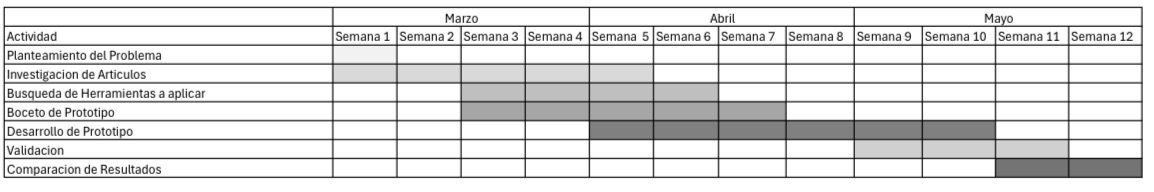
\includegraphics[scale=.4]{cronogramaFV2.jpeg} %Poner el nombre de tu imagen
    \caption{Cronograma de actividades}
    \label{fig:cron}
\end{figure}

\clearpage
\bibliography{mybibliography.bib} %Se asume que se tiene el archivo mybibliography.bib
\end{document}